\label{sec:02Preliminarystudies}
\section{Preliminary studies}

\subsection{Data visualization}
We have worked on the closed price values of the CAC40 index as data, downloaded from the website finance.yahoo.com.\\
We started by displaying the data and trying to understand them, in order to be relevant in our way to study and model them.

\FloatBarrier
\begin{figure}[!htbp]
  \centering
  \includegraphics[width=\textwidth]{img/Plot1.eps}
  \caption{CAC40 values from 1998 to April 2018}
\end{figure}
\FloatBarrier

As we can see in the Figure 1, data seems to have a specific behavior during the period from 1998 to 2010, and a different evolution during the period from 2010 to 2018. In the first period indeed, data has known a high peak then a significant drop throughout 5-6 years, two times in a row, whereas in the second period they are just slightly increasing over time. \\
The drop which occurred in 2001 is because stock prices took a sharp downturn (some say "stock market crash" or "the Internet bubble bursting") in stock markets across the United States, Canada, Asia, and Europe. After recovering from lows reached following the September 11 attacks, indices slid steadily starting in March 2002, with dramatic declines in July and September leading to lows last reached in 1997 and 1998. \\
Regarding the drop from the middle of 2007, it can be explained by the global financial crisis of 2007-2008. \\
Given the fact that data evolution during the first period seems to be ruled by exceptional events, and the behavior or "stability" during the second one seems different, we decided to focus our work on data from 2012 to 2018 so our model will not be affected by events named above.

\FloatBarrier
\begin{figure}[!htbp]
  \centering
  \includegraphics[width=\textwidth]{img/Plot3.eps}
  \caption{CAC values from 2012 to April 2018, with train \& validation regions}
\end{figure}
\FloatBarrier

In practice, we have stored the data in a time series object, so we can use R’s many functions for analyzing time series data. We use the $ts()$ function in R to do that. \\
Since our time series data set has been collected at regular intervals, we specify the number of times that data was collected per year by using the $frequency$ parameter in the $ts()$ function. We set $frequency = 256$ since we have in average 256 data collected per year. \\
We also specify the first year that the data was collected, and the first interval in that year, by using the $start$ parameter in the $ts()$ function. Thus we set $start=c(2012,1)$. \\
We also set $end=c(2016,256)$ to work on data to the end of 2016, and thus we defined a period from 2012 to the end of 2016 to train our model, before testing it on the period from 2017 to 2018. It means that we will analyze how the model fit by comparing its forecast with the observed data over the period from 2017 to 2018 (the validation period), and only after this step we will perform forecasting.
 

\subsection{Data manipulation}
Our dataset leads us to reformat dates (from French to American format), and to remove null values and outliers. \\
Sometimes indeed we may have some outliers in our data, or simply null values, which can bring errors through analyses. To figure this out, we can use the $tsclean()$ function to detect and remove them. Here, we have manually removed null values in the data file, and comparison between data before and after the use of $tsclean()$ shows that there is apparently no outliers. \\


\subsection{Summary}
We can easily access to some statistical information about the serie, thanks to the R function summary(). Find in Tables 2 and 3 minimum, maximum and mean values, as well as the median and quartiles of our time series. \\

\FloatBarrier
\begin{table}[!htbp]
  \centering
  \begin{tabular}{|c c c|} 
  \hline
  Min. & Mean & Max. \\
  \hline
  2950 & 4386 & 5542 \\ 
  \hline
  \end{tabular}
  \caption{Mean and border values of the serie}
\end{table}
\FloatBarrier
\begin{table}[!htbp]
   \centering
   \begin{tabular}{|c c c|} 
   \hline
   1st Quart. & Median & 3rd Quart. \\
   \hline
   3982 & 4401 & 4911 \\ 
   \hline
  \end{tabular}
  \caption{Median and quartiles of the serie}
\end{table}
\FloatBarrier

\subsection{First analyses}
Following teacher's instruction, we used log transformation on the data.
Indeed, log transformation is usually used for several reasons :
\begin{enumerate}
\item to transform a multiplicative model to an additive model (see farther).
\item to remove unequal variances or exponential growth in the series.
\item in finance, for convenience (if price is log-normally distributed, or to approximate raw returns when returns are small, or for other mathematical and numerical advantages).
\end{enumerate}
However it might be not necessary here because as we can see with Figures 2 and 3, we have the same shape with and without the log transformation. \\

In Figure 3 we used \textit{lm()} function to carry out a regression, and \textit{abline()} function to plot it. \\
It shows that price is globally increasing over time, and also that this time series could probably be described using an \textbf{additive model}, since the random fluctuations in the data are roughly constant in size over time. \\
\\
\FloatBarrier
\begin{figure}[!htbp]
  \centering
  \includegraphics[width=\textwidth]{img/Fig3.eps}
  \caption{Log of the price}
\end{figure}
\FloatBarrier

\subsection{Data decomposition \& Stationarity}

\subsubsection{Additive and multiplicative models}
As we have seen in the first part of this report, ARMA modeling with time series requires series to be stationary. \\
We can deduce from Figure 3 that our series is not stationary, and the Augmented Dickey-Fuller Test \cite{banerjee1993co,said1984testing} with R confirms that we can't reject the null hypothesis of non-stationarity (p-value from the test is too high, see Listing 1). \\

\begin{lstlisting}[language=R, caption=First test of stationarity]
	Augmented Dickey-Fuller Test

data:  lserie
Dickey-Fuller = -2.5076, Lag order = 10, p-value =
0.3634
alternative hypothesis: stationary
\end{lstlisting}

To figure out this issue, we need to make some data transformations, like removing the seasonality, the trend, and/or differencing the serie. \\

Actually, time series are made up of four components:
\begin{enumerate}
  \item $S_t$: the seasonal component, which refers to fluctuations in the data related to calendar cycles.
  \item $T_t$: the trend component, which is the overall pattern of the series.
  \item $C_t$: the cyclical component, which consists of decreasing or increasing patterns that are not seasonal. Usually, trend and cycle components are grouped together. Trend-cycle component is estimated using moving averages (see farther).
  \item $E_t$: the error or irregular component, which is the part of the series which can't be attributed to other components.
\end{enumerate}
And we distinguish 2 kinds of decomposition for a time series :
\begin{enumerate}
  \item the additive decomposition: $Y_t = S_t + T_t + C_t + E_t$, where $Y_t$ is the data at time $t$.
  \item the multiplicative decomposition: $Y_t = S_t * T_t * C_t * E_t$.
\end{enumerate}

\subsubsection{Seasonality of the time series}
According to Figure 3 (above), there is no apparent seasonality in the data over this period, neither apparent cycle. Thus we could skip the seasonal adjustment and work on the trend of the time series. \\
On top of that, removing seasonality is not a mandatory step here, since with R we can build an ARMA model with orders (p,q) for the deseasonal part, and orders (P,Q) for the seasonal component. Such orders can be easily detected with the function \textit{auto.arima()}. \\
But for practice, this step will still be performed.

\subsubsection{Trend of the time series}
We can approach the trend component of our time series by taking successive orders of moving averages.\\
Note that the moving average in this context is distinct from the MA(q) component in the  ARIMA definition you have seen previously. Moving average MA(q) as part of the ARIMA framework refers to error lags and combinations, whereas the summary statistic of moving average refers to a data smoothing technique. \\
The wider the window of the moving average, the smoother original series becomes. In our case, we can take weekly, monthly or annual moving average, and then approximate the trend of the time series, as Figures 4 5 and 6 show.
\\
\FloatBarrier
\begin{figure}[!htbp]
  \centering
  \includegraphics[width=\textwidth]{img/Fig4.eps}
  \caption{Order 5 (weekly) moving average}
\end{figure}
\FloatBarrier
\FloatBarrier
\begin{figure}[!htbp]
  \centering
  \includegraphics[width=\textwidth]{img/Fig5.eps}
  \caption{Order 21 (monthly) moving average}
\end{figure}
\FloatBarrier
\FloatBarrier
\begin{figure}[!htbp]
  \centering
  \includegraphics[width=\textwidth]{img/Fig6.eps}
  \caption{Order 256 (annual) moving average}
\end{figure}
\FloatBarrier

\subsubsection{Decomposition of the time series}
With R, \textit{stl()} function allows us to decompose time series in 3 components :
\begin{enumerate}
  \item a seasonal component
  \item a trend-cycle component
  \item a remainder, or error component
\end{enumerate}

\FloatBarrier
\begin{figure}[!htbp]
  \centering
  \includegraphics[width=\textwidth]{img/Fig7.eps}
  \caption{Decomposition of the series}
\end{figure}
\FloatBarrier

As we can see in the Figure 7, the trend-cycle component looks like our approximation of the trend with moving averages (see Figure 6). \\
We also notice that the seasonal component is not null but very low compared with other components, and then it might be negligible, as we deduced before.\\

From now let's work with the log-transformed series as the time series under study. \\
We have two ways to remove seasonality from our time series:
\begin{enumerate}
\item Performing $Y_t^S = Y_t - S_t$, where $Y_t$ is the original data, and $S_t$ the seasonal component (because we have an additive model here, otherwise we would perform $\frac{Y_t}{S_t}$).
\item Using \textit{seasadj()} function from \textit{forecast} package, which removes the seasonal component given the result of the \textit{stl()} function as parameter.
\end{enumerate}
Both methods give the same result, available in Figure 8 \\

\FloatBarrier
\begin{figure}[!htbp]
  \centering
  \includegraphics[width=\textwidth]{img/Fig7b.eps}
  \caption{Deseasonalized Series}
\end{figure}
\FloatBarrier

For the trend component, we also have two ways to remove it :
\begin{enumerate}
\item Performing $Y_t^{S,T} = Y_t^S - T_t$, where $Y_t^S$ is the deseasonalized time series, and $T_t$ the trend component (here trend-cycle component).
\item Using function \textit{diff()}.
\end{enumerate}

With R, \textit{diff()} function returns, given a time series $(X_t)$ as parameter, a time series $(Z_t)$ which is the differences between all consecutive values of $(X_t)$. In other words, $Z_t = X_{t+1} - X_t$. If $(X_t)$ is not stationary but $(Z_t)$ is, then we can identify an ARMA($p_z$,$q_z$) model for $(Z_t)$, which will be an ARIMA($p_z$,$1$,$q_z$) for $(X_t)$. Indeed, each use of the \textit{diff()} transformation increments by 1 the order $d$. If it happens that $d=1$ is not enough to get a stationary series, then we try with higher values of $d$ until the series is stationary. \\
Here we decided to first try to remove the trend-cycle component of the deseasonalized series, before taking an interest in the differentiated series. The result is available in Figure 9 below.

\FloatBarrier
\begin{figure}[!htbp]
  \centering
  \includegraphics[width=\textwidth]{img/Fig7c.eps}
  \caption{Random Part of the Series}
\end{figure}
\FloatBarrier

\subsubsection{Stationarity of the decomposed time series}

From Figure 9, we can see that our series seems to be stationary, because data values oscillate with a steady variance around the mean of 0.
In addition, the Augmented Dickey-Fuller test with R confirms that we can reject the null hypothesis of non-stationarity since the p-value from the test is lower than 0.05 (Listing 2). \\

\begin{lstlisting}[language=R, caption=Final test of stationarity]
	Augmented Dickey-Fuller Test

data:  random_stl
Dickey-Fuller = -4.4514, Lag order = 10, p-value = 0.01
alternative hypothesis: stationary
\end{lstlisting}